\chapter{Two-Particle Simulations}\label{Sec:TwoParticleResults}

\section{Flat Band Initial State}\label{Sec:HexagonResults}

This section presents two-particle simulations with both particles initially in the same localised flat band hexagon state (as depicted in Fig. \ref{Fig:Hexagon_Eigenstate} for a single particle). In terms of the creation operators, this is:
\begin{subequations}\label{Eq:Hexagon_Initial_State_and_Operator}
    \begin{equation}\label{Eq:Hexagon_Initial_State}
        |\Psi(t=0)\rangle=\frac{1}{\sqrt{2}}(h_{i}^{\dag})^2|0\rangle
    \end{equation}
    \begin{equation}\label{Eq:Hexagon_Operator}
        h_{i}^\dag=\sum_{l}\frac{(-1)^{l}}{\sqrt{6}}b_{l}^{\dag}
    \end{equation}
\end{subequations}
where $l$ indexes the six sites of hexagon $i$. Eq. \ref{Eq:Hexagon_Initial_State} will subsequently be referred to as the `hexagon initial state'. Since this state is stationary for $U=0$, the mobility of the particles is solely due to interactions lifting the flat band degeneracy. If the particles were instead initialized on two non-overlapping hexagons, there would be no interaction energy and hence the particles would remain stationary. 

Simulations of two interacting particles initially on the same site are presented in Appendix \ref{App:SingleSite_2p}. These are directly comparable to Section \ref{Sec:SingleParticleResults}; however, the hexagon initial state more effectively illustrates the effect of interactions specifically within the flat band, without the complications of density from the dispersive bands.

\begin{figure}[p!]
    \centering
    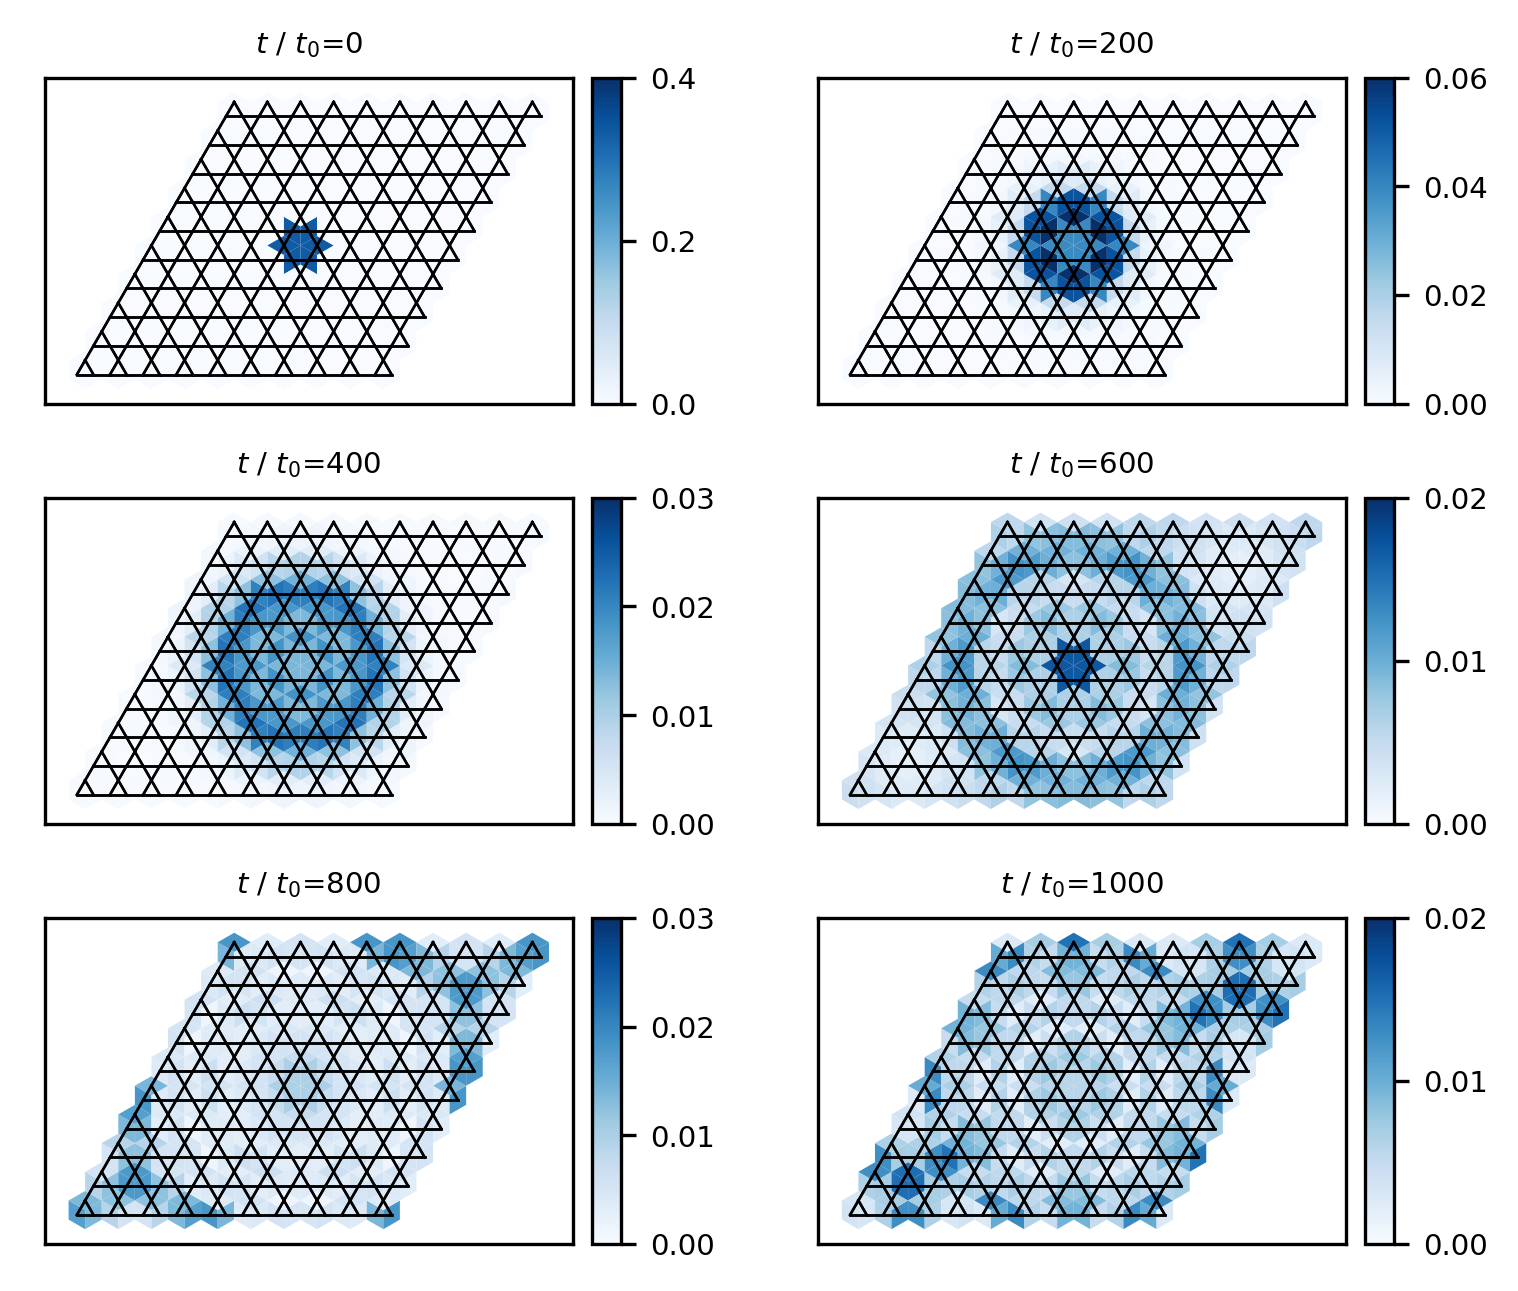
\includegraphics[width=\textwidth]{Figures/Hexagon_Evolution}
    \caption{Time-evolution of density $\langle n \rangle$ from the hexagon initial state, for $U/J=0.1$. The lattice size, $10\times10$ unit cells, is the same throughout Section \ref{Sec:TwoParticleResults} unless stated otherwise. The colour scale varies between plots.}
    \label{Fig:Hexagon_Evolution}
\end{figure}

\newpage

\subsection{Dynamical Behaviour and Interaction-Shifted Eigenspectrum}\label{Sec:HexagonQualitative}

The qualitative behaviour when evolving from the hexagon initial state is illustrated in Fig. \ref{Fig:Hexagon_Evolution}. With $0<U\ll J$, most of the density spreads symmetrically as a single wavepacket, with little dispersion; a small amount remains stationary in the original hexagon. 

This can be explained from the shifts to the energy eigenvalues by the interactions. Fig. \ref{Fig:Energy_Shifts} shows the numerically obtained eigenvalues for pairs of particles, relative to the unperturbed flat band energy, plotted against the magnitude of the total momentum $q=|\textbf{q}|$ of the eigenstate. The numerical eigenvectors were projected onto the two-particle flat band Bloch states $|\textbf{k}_1\rangle |\textbf{k}_2\rangle$ (direct products of Eq. \ref{Eq:FBBlochState}) to obtain the contributing values of $\textbf{q}=\textbf{k}_1+\textbf{k}_2$ in each case. As predicted in Section \ref{Sec:WeakInteractionTheory}, the eigenstates are associated with certain $\textbf{q}$ values. Due to the six-fold rotational symmetry of the kagome lattice, most eigenstates are six-fold degenerate, depending only on the magnitude $q$ not the direction of $\textbf{q}$; Fig. \ref{Fig:Energy_Shifts} does not show this degeneracy explicitly. 

\vspace{0.5cm}

\begin{figure}[ht]
    \centering
    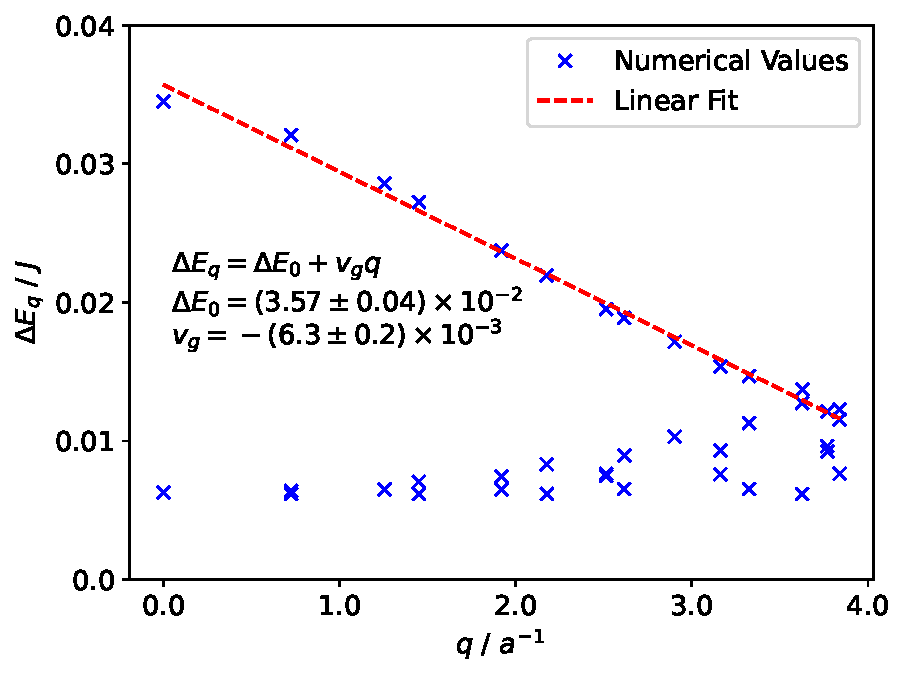
\includegraphics[width=10cm]{Figures/FB_Energy_Shifts}
    \caption{Numerically obtained flat band eigenvalues for $U/J=0.1$, relative to the flat band energy, against the magnitude of the total momentum of the eigenstate. The unperturbed eigenvalues of non-overlapping flat band states are not plotted. A linear fit, giving the group velocity, is performed to the highest-energy eigenvalues at each $q$.}
    \label{Fig:Energy_Shifts}
\end{figure}

For the hexagon initial state, $\approx 80\%$ of the density occupies the highest-energy eigenstates whose energy is linear with $q$ in Fig. \ref{Fig:Energy_Shifts}. The linear gradient explains the mobile density remaining together as a single wavepacket in Fig. \ref{Fig:Hexagon_Evolution}; all eigenstates have the same group velocity magnitude. Moreover, the isotropic spreading is consistent with $\Delta E_q$ depending only on $q$, not the direction of $\textbf{q}$. 

The remaining density not occupying these highest-energy states is divided between the lower-energy pair states in Fig. \ref{Fig:Energy_Shifts}, unperturbed (non-overlapping) flat band states, and states from the dispersive bands. The lower pair energies are almost dispersionless, which, along with the unperturbed flat band states, explains the stationary and slowly-propagating density visible in the original hexagon and surrounding area at late times in Fig. \ref{Fig:Hexagon_Evolution}. The dispersive states are fast-propagating, and give small fluctuations.

\vspace{1cm}

\subsection{Dependence on Interaction Strength}\label{Sec:HexagonQuantitative}

For systems with larger $U$, the interaction energy shifts and group velocities are greater. The density in the original hexagon, denoted $n_{h}$, therefore decays more quickly, as Fig. \ref{Fig:Original_Hexagon_Density} shows. For $U/J=0.5$, a peak occurs around $t=300\,t_0$, due to the wavepacket passing completely around the lattice (with its periodic boundary conditions) and recombining in the original hexagon after a certain `recombination time'. Fig. \ref{Fig:Original_Hexagon_Density} motivates two methods of quantifying the dependence of the particle mobility on $U$: the decay time of $n_{h}$, and the recombination time (which is inversely proportional to the group velocity). Fig. \ref{Fig:Original_Hexagon_Density} also illustrates that the behaviour becomes more complicated for $U/J\gtrsim 1$. Here, $H_U$ cannot be considered a weak perturbation to $H_J$, so the hexagon initial state has a mixed character of the flat and dispersive bands. There are therefore components with high group velocities, which rapidly propagate around the lattice, causing the complex fluctuations in $n_{h}$.

\newpage

\begin{figure}[ht!]
    \centering
    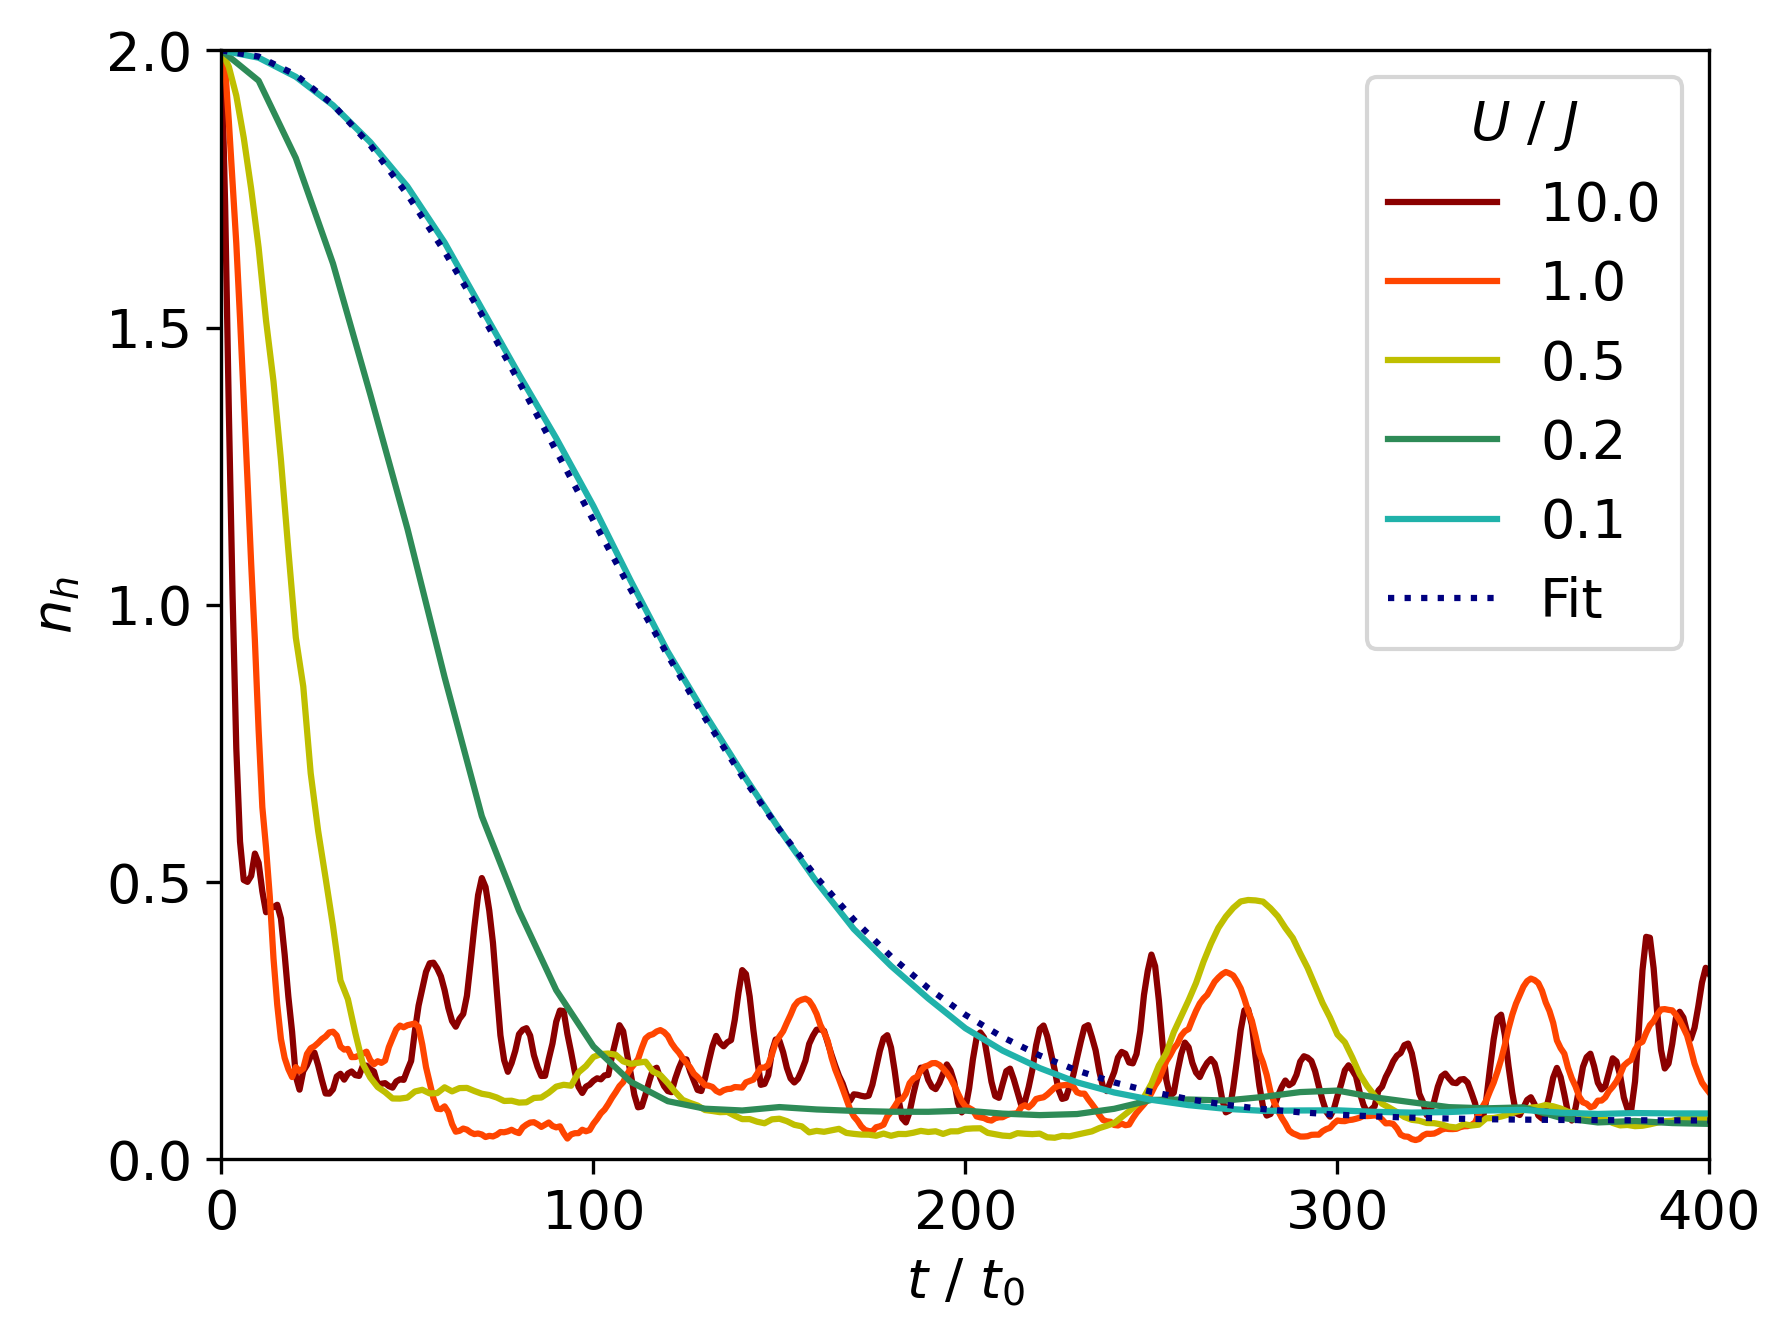
\includegraphics[width=10cm]{Figures/Original_Hexagon_Density}
    \caption{Time-evolution of density within the original hexagon, $n_{h}$, from simulations with the hexagon initial state, for various interaction strengths. An example curve fitted to the $U/J=0.1$ data is also plotted (navy, dotted).}
    \label{Fig:Original_Hexagon_Density}
\end{figure}

For $U/J\lesssim1$, $n_{h}$ can be accurately modelled by a Gaussian fitting the initial decay, plus a constant accounting for the stationary density:
\begin{equation}\label{Eq:Gaussian_Fit}
    n_{h}(t) = (2-c)\exp{\left(-\frac{1}{2}\left(\frac{t}{\tau}\right)^2 \right) } + c
\end{equation}
The prefactor $2-c$ ensures $n_{h}(t=0)=2$, consistent with the initial state. Fig. \ref{Fig:Decay_Time} shows the dependence of the fitted parameter $\tau$ on $U$. For $U\ll J$, fitting a power law gives $\tau \appropto U^{-1}$. This is consistent with $H_U$ being a weak perturbation to $H_J$, causing energy shifts (and therefore particle velocity) $\propto U$ to leading order. The constant $c$ did not vary significantly with $U$. Fig. \ref{Fig:Recombination_Time} shows the recombination time $t_r$ against $U$. As with the decay time, $t_r \appropto U^{-1}$, implying that $v_g\propto U$. In both plots, higher order effects (deviations from the fitted power laws) are visible beyond $U/J \gtrsim 0.1$.

The group velocity magnitude obtained from the eigenspectrum for $U/J=0.1$ (Fig. \ref{Fig:Energy_Shifts}) is $|v_g| = (6.3 \pm 0.2)\times 10^{-3}\: a/t_0$ (the sign is unimportant). Using the expression for $t_r$ from Fig. \ref{Fig:Recombination_Time} and the lattice width $L=10\,a$ gives the simulation group velocity as $|v_g| = L/t_r=(6.33 \pm 0.05)\times 10^{-3} \: a/t_0$, demonstrating excellent consistency.

\begin{figure}[ht!]
    \centering
    \sidesubfloat[]{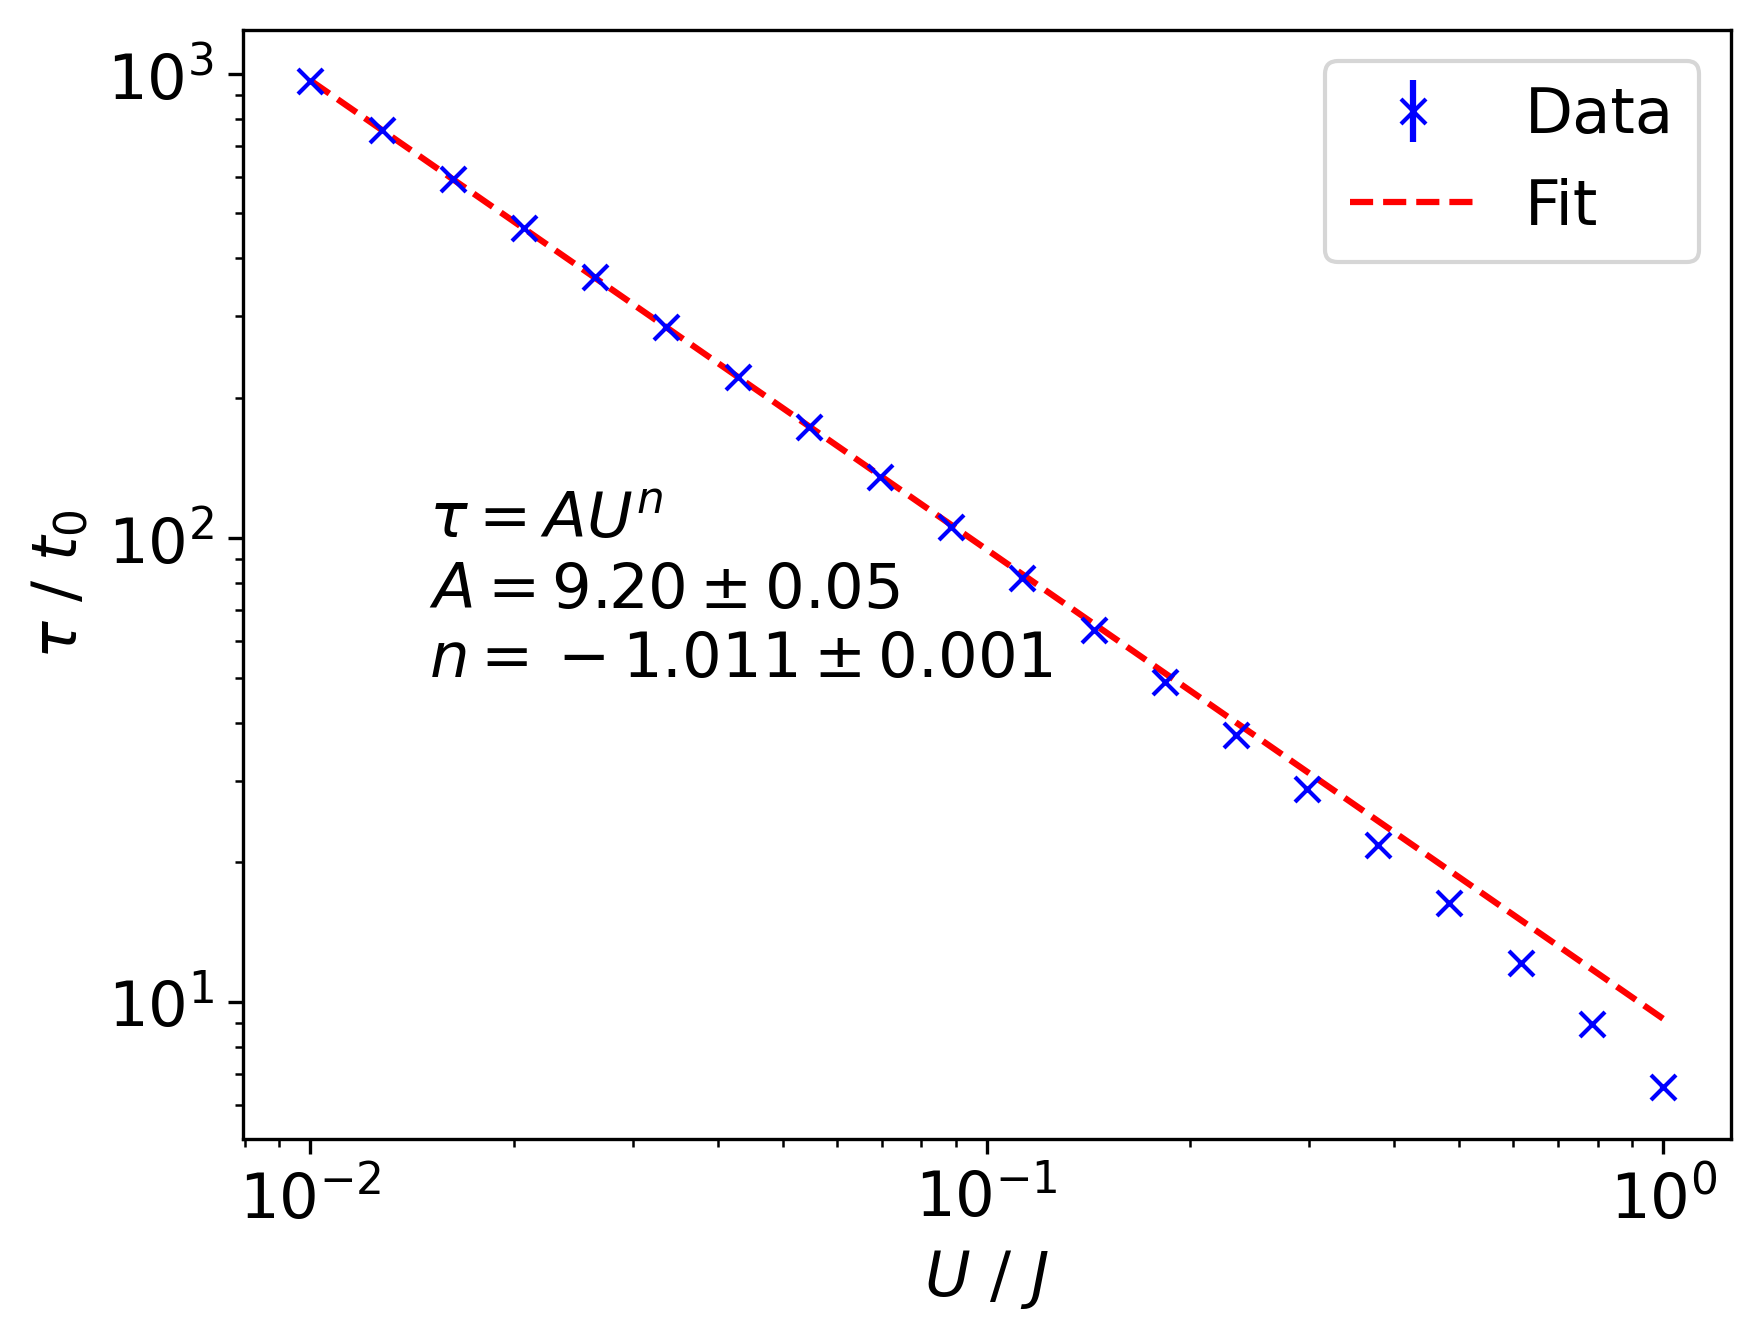
\includegraphics[height=5.6cm]{Figures/Decay_Time}\label{Fig:Decay_Time}}\hfill
    \sidesubfloat[]{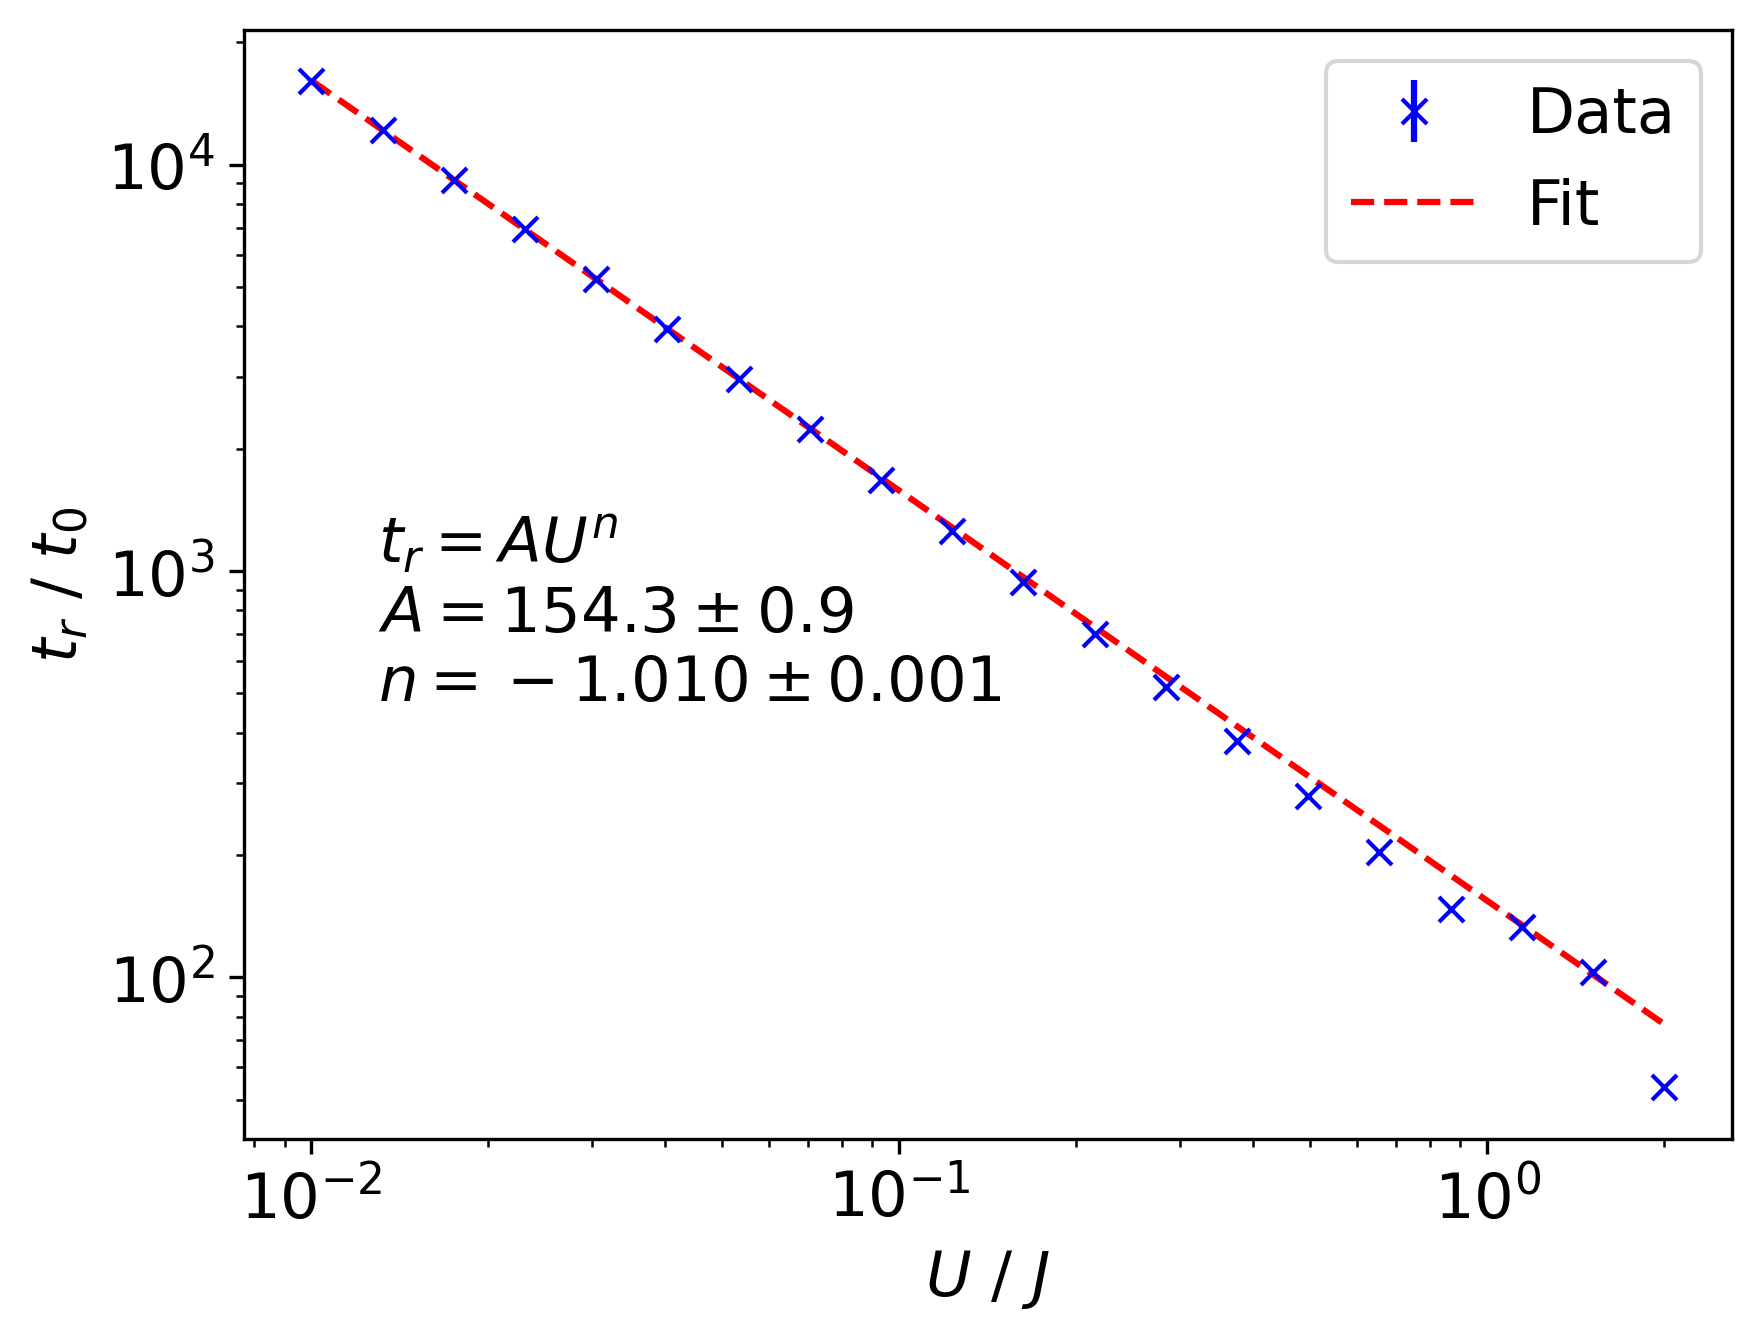
\includegraphics[height=5.6cm]{Figures/Recombination_Time}\label{Fig:Recombination_Time}}
    \caption{(a) Decay time and (b) recombination time of density in the original hexagon, determined from simulations with the hexagon initial state, plotted against interaction strength. Power law fits to the data for $U/J\leq 0.1$ are close to the predicted $U^{-1}$ relationships. The data are only plotted for $U/J\lesssim 1$ where Eq. \ref{Eq:Gaussian_Fit} is a good fit to $n_{h}$, and $t_r$ is clearly identifiable.}
    \label{Fig:Decay_and_Recombination_Time}
\end{figure}
\text{}%\vspace{0.4cm}

\subsection{OPDM and Flat Band Projection}\label{Sec:FBProjection}

The behaviour throughout Section \ref{Sec:HexagonResults} has been explained within a weak-perturbation framework: direct products of single-particle flat band states are good two-particle eigenstates, whose mobility is due to interactions lifting their degeneracy, rather than an admixture of states from dispersive bands. This section further verifies this using the one-particle density matrix (OPDM). Following the methodology in \cite{Bera,Lezama}, the OPDM is defined as:
\begin{equation}\label{Eq:OPDM}
    \rho_{ij}(t)=\langle \Psi(t)|b_i^{\dag}b_j|\Psi(t)\rangle
\end{equation}
The eigenstates of the OPDM $\{|\phi_\alpha\rangle\}$ are the `natural single particle orbitals' of the system, and the corresponding eigenvalues $\{n_\alpha\}$ their occupancies; $\sum_{\alpha} n_{\alpha}=\text{Tr}(\rho)=N$, the number of particles in the system. The total occupancy of single-particle flat band states, $N_{\text{FB}}$, is given by the trace of the OPDM after projecting onto the flat band:%\newpage\noindent
\begin{subequations}
    \begin{equation}
        N_{\text{FB}}=\text{Tr}(\hat{P}\rho\hat{P})
    \end{equation}
    \begin{equation}
        \hat{P} = \sum_{\textbf{k}}|\textbf{k}\rangle \langle \textbf{k}|
    \end{equation}
\end{subequations}
where $|\textbf{k}\rangle$ are the single-particle flat band Bloch states (Eq. \ref{Eq:FBBlochState}). 

 In general, $N_{\text{FB}}$ is not constant in time for states which are not eigenstates of $\hat{P}$; therefore, the time-averaged $\overline{N}_{\text{FB}}$ is plotted in Fig. \ref{Fig:FB_Occupancy}. $\overline{N}_{\text{FB}}\approx2$ and is almost constant for $U/J\ll 1$, confirming that direct products of single-particle flat band states are good two-particle eigenstates. In fact, as Fig. \ref{Fig:NFB_Occupancy} shows, the `non-flat-band occupancy', $2-\overline{N}_{\text{FB}}$, is $\appropto U^2$ for weak interactions. This is consistent with an admixture of dispersive states within first-order perturbation theory, with amplitude $\propto U$, and therefore occupancy $\propto U^2$.

For $U\gg J$, $\overline{N}_{\text{FB}}$ does not decrease all the way to 2/3 as might be expected from an equal occupancy of all bands. This is because, regardless of the interaction strength, the hexagon initial state is inevitably composed of exact eigenstates which share certain common features with the flat band states, such as alternating signs between sites. Nevertheless, the flat band states are clearly no longer good eigenstates for $U/J\gtrsim 1$, as stated previously when interpreting the system behaviour in this limit.

\vspace{1cm}

\begin{figure}[ht]
    \centering
    \sidesubfloat[]{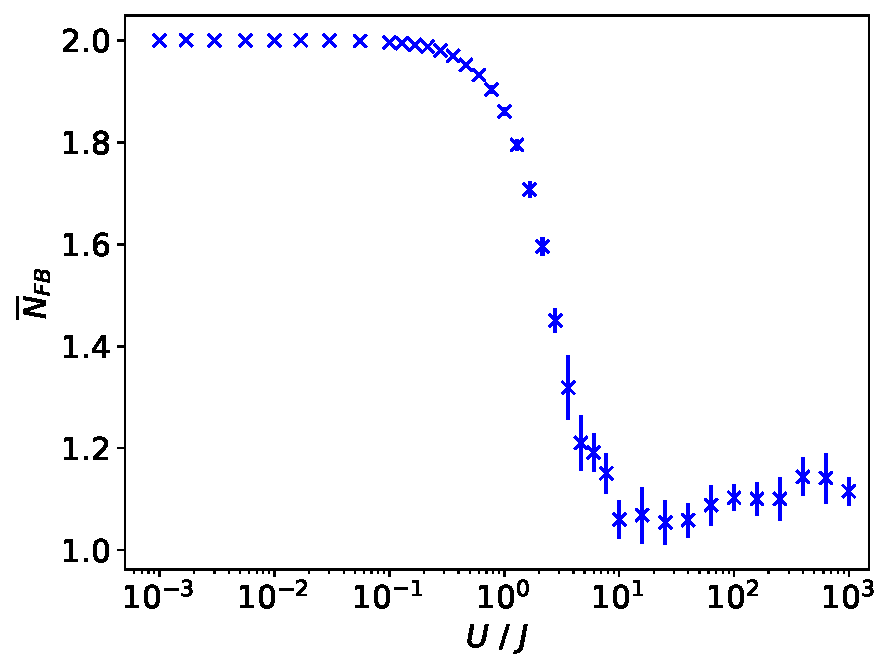
\includegraphics[height=5.6cm]{Figures/FB_Occupancy}\label{Fig:FB_Occupancy}}\hfill
    \sidesubfloat[]{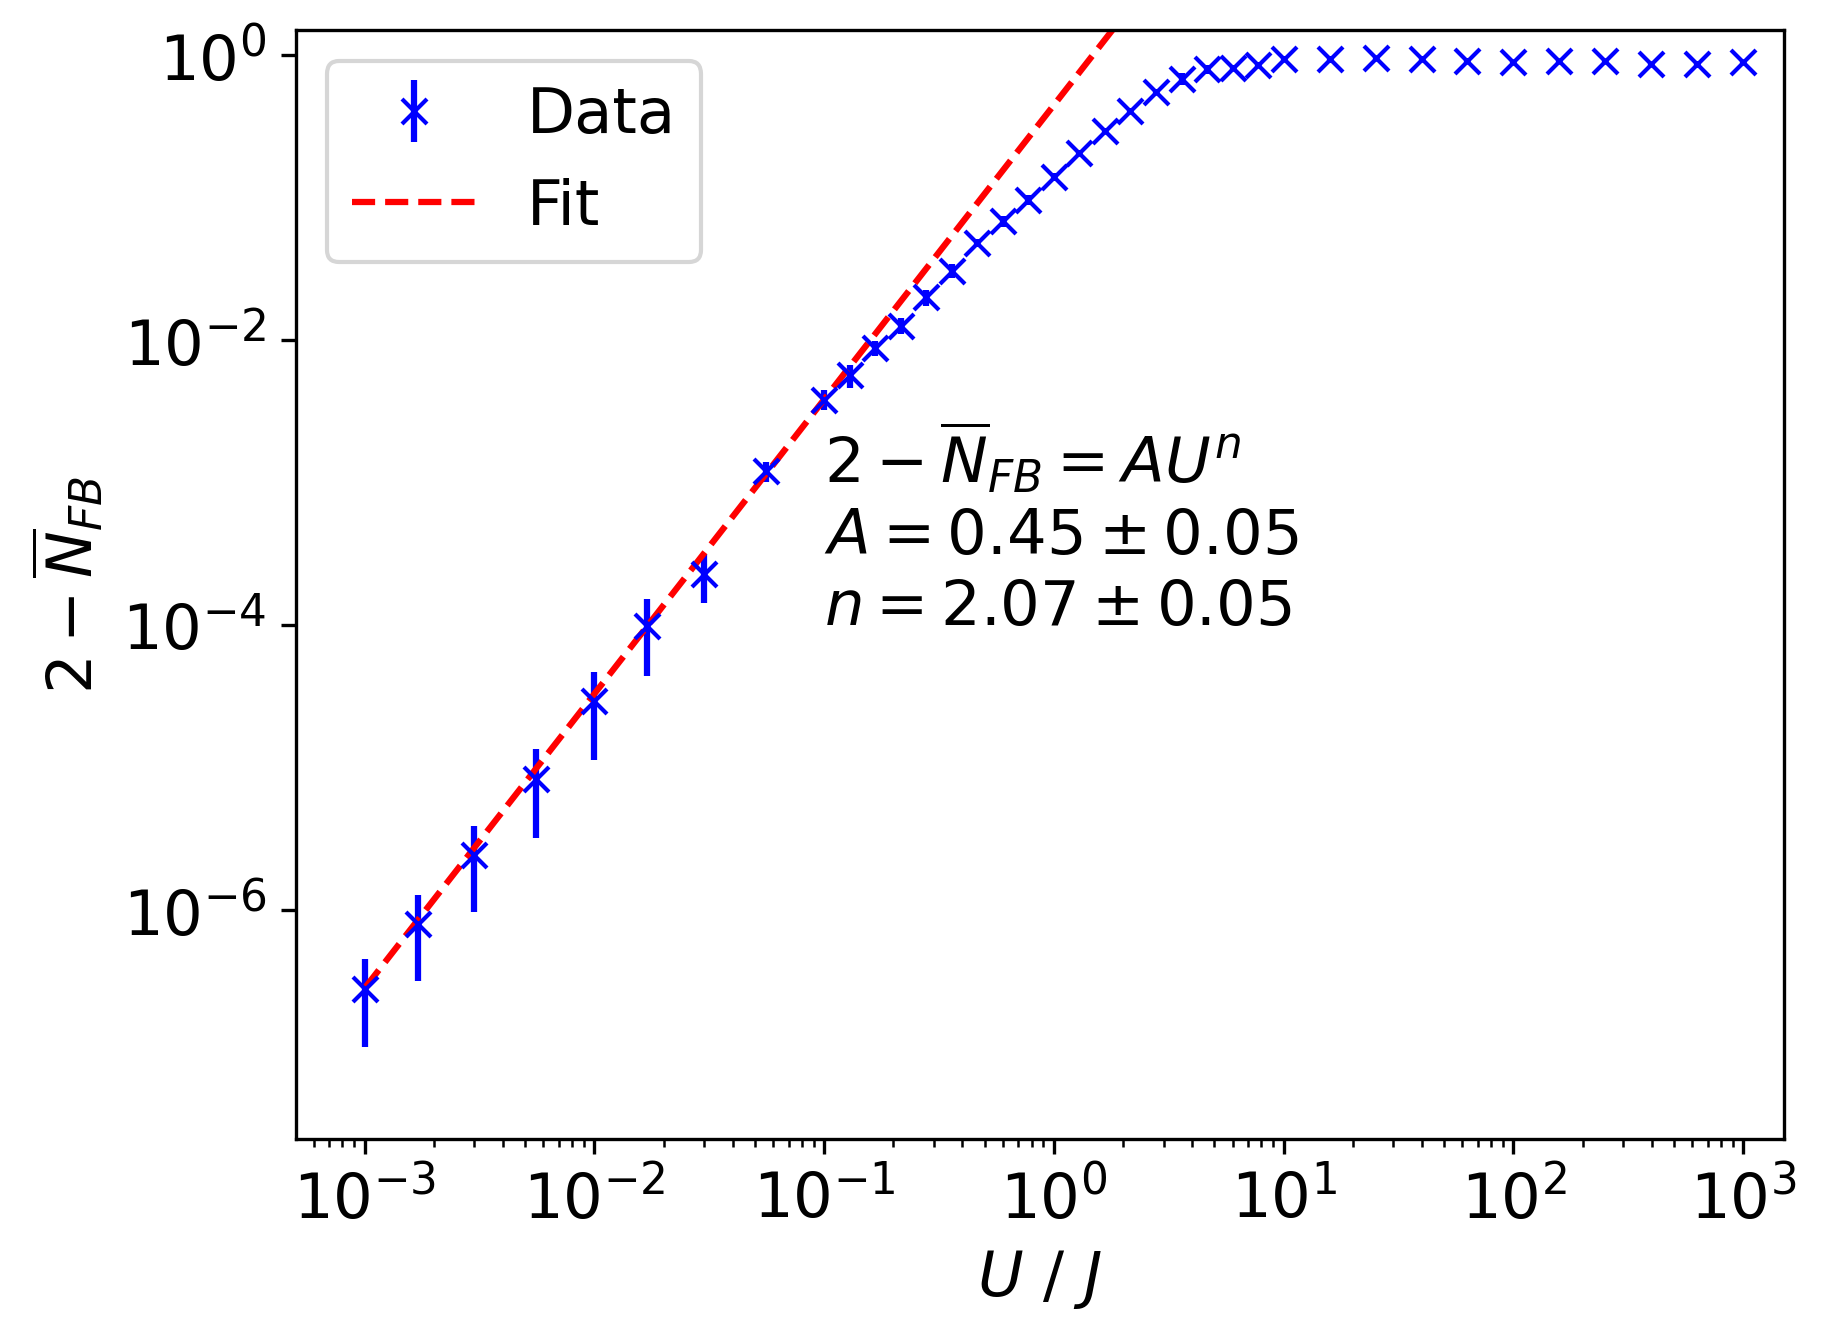
\includegraphics[height=5.6cm]{Figures/NFB_Occupancy}\label{Fig:NFB_Occupancy}}
    \caption{Time-averaged (a) flat-band occupancy and (b) non-flat-band occupancy against interaction strength, from simulations with the hexagon initial state. Error bars show the standard deviation of fluctuations. The power law fit in (b) is performed to the data for $U\leq 0.1$.}
    \label{Fig:FB_NFB_Character}
\end{figure}

\section{Strong Interactions}\label{Sec:Strong_Interactions}

For strong interactions, $U\gg J$, the eigenspectrum divides into a scattering band and a doublon band, as discussed in Section \ref{Sec:DoublonTheory}. In this section, the theoretical predictions are compared to numerical results, and the resulting dynamical behaviour is examined, for systems with $U/J=100$. 

\subsection{Eigenspectrum}\label{Sec:Doublon_Eigenspectrum}

Fig. \ref{Fig:Doublon_Eigenspectrum} shows the doublon band eigenvalues, which agree closely with those of a single particle with the theoretical effective doublon hopping coefficient from Eq. \ref{Eq:DoublonHamiltonian}. In Appendix \ref{App:DoublonHigherOrder}, it is verified that discrepancies are due to higher order hopping processes, giving energy shifts $\propto \frac{J^3}{U^2}$.

The scattering band eigenvalues are shown in Fig. \ref{Fig:Scattering_Eigenspectrum} and compared to the non-interacting case. The non-interacting spectrum shows various plateaus of degenerate eigenstates due to the rotational symmetries of the system. With interactions, the degeneracies are partially lifted, for the eigenstates in which the particles overlap in real space. The scattering eigenvalues are virtually unaltered for systems with greater $U$.

\begin{figure}[ht]
    \centering
    \sidesubfloat[]{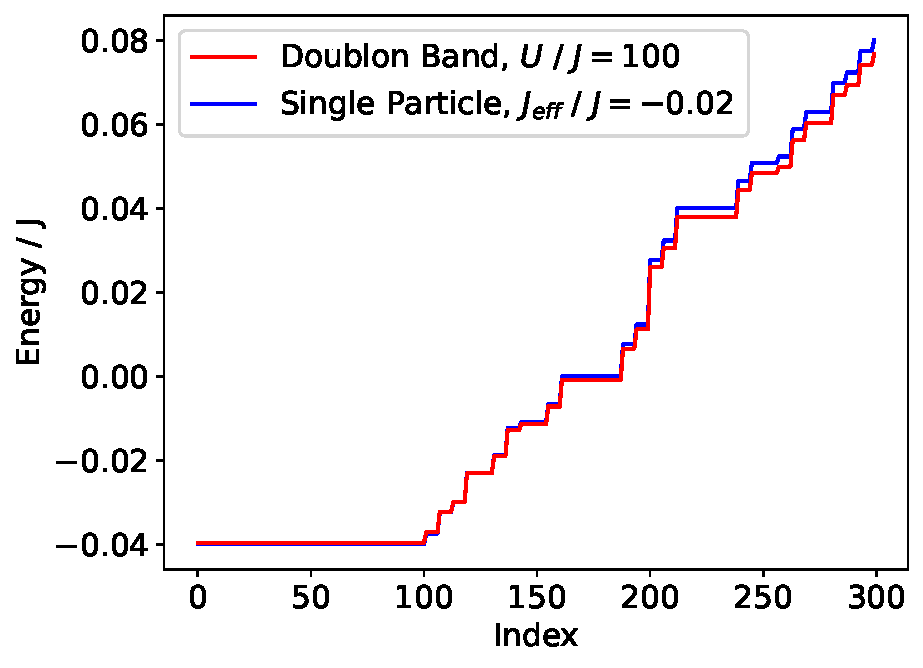
\includegraphics[height=5.6cm]{Figures/Doublon_Eigenspectrum}\label{Fig:Doublon_Eigenspectrum}}\hfill
    \sidesubfloat[]{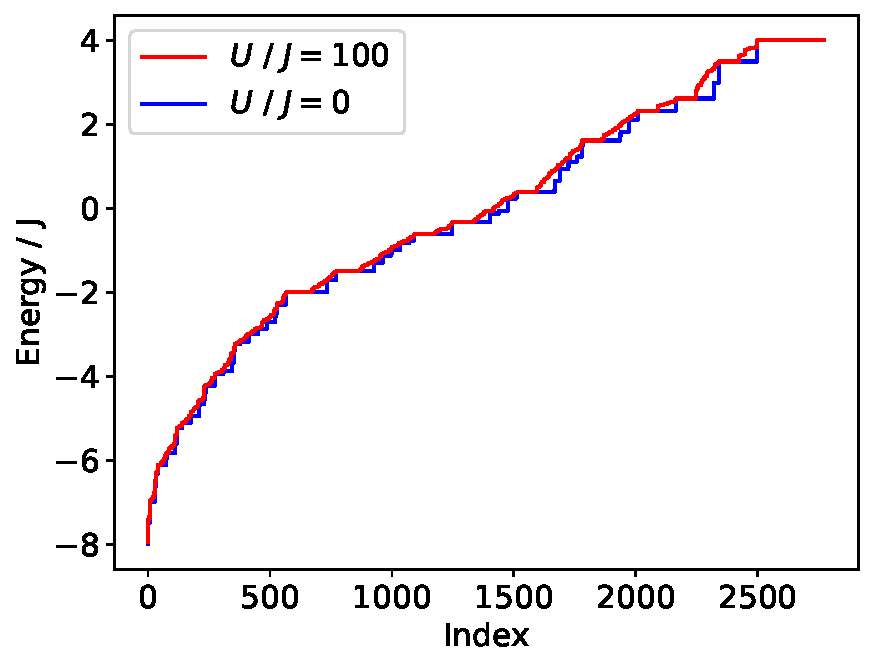
\includegraphics[height=5.6cm]{Figures/Scattering_Eigenspectrum}\label{Fig:Scattering_Eigenspectrum}}
    \caption{Numerically obtained eigenvalues in the strongly-interacting limit, plotted in ascending order (the index is physically meaningless). (a) Doublon band for a 10$\times$10 unit cell system, shifted down by $E_0$, compared to single-particle eigenspectrum with $J=J_{\text{eff}}$. $E_0$ and $J_{\text{eff}}$ are defined in Eq. \ref{Eq:DoublonHamiltonian}. (b) Scattering band for 5$\times$5 unit cell systems, for strongly- and non-interacting cases.}
    \label{Fig:Scattering_Doublon_Eigenspectrum}
\end{figure}
%Add note - scattering eigenspectrum doesn't change much for stronger interactions?

\subsection{Dynamical Behaviour}\label{Sec:Strong_Interaction_Dynamics}

For $U\gg J$, doublons cannot separate, and instead propagate through the lattice as a composite particle; this is explicitly verified in Appendix \ref{App:Doublon_Fraction}. Fig. \ref{Fig:Doublon_SingleSite_Evolution} shows the simulation results with two particles initially in a doublon state, $|\Psi(t=0)\rangle=\frac{1}{\sqrt{2}}(b_{i}^{\dag})^2|0\rangle$. The density in the original site $i$ is plotted against time, and compared to the density simulated for a single particle with the theoretical $J_{\text{eff}}$ of the doublon (the constant $E_0$ does not affect the physical behaviour). The data appear identical up to a re-scaling of the time axis. This is due to the discrepancies between the doublon and effective single-particle eigenspectra in Fig. \ref{Fig:Doublon_Eigenspectrum}. These are linear with energy (see Appendix \ref{App:DoublonHigherOrder}); this linear scaling between the frequency spectra therefore causes the re-scaling of the real-time behaviour. 

Fig. \ref{Fig:Scattering_Evolution} shows the simulation results of two particles initially on different lattice sites, $|\Psi(t=0)\rangle=b_{i}^{\dag}b_{j}^{\dag}|0\rangle$ (a scattering band state). The density in one of the initial sites is plotted against time. For $U/J=0$, there are large fluctuations due to degenerate eigenstates interfering in phase. With interactions, this degeneracy is partially lifted (see Fig. \ref{Fig:Scattering_Eigenspectrum}), and the fluctuations are less pronounced. This can be intuitively understood as interacting particles repelling each other and spreading uniformly throughout the lattice, instead of propagating together in wavepackets, causing large instantaneous density fluctuations. 

\vspace{0.5cm}

\section{Particle Separation}\label{Sec:ParticleSeparation}

This section examines the variation of the particle separation during the simulations. This captures several features of the different behaviour regimes discussed above, and the transition between them. For weak interactions, it is verified that particles are only mobile as a bound pair (since spatially-separated states are not shifted in energy); and for strong interactions, the division of doublon and scattering states is further evidenced.

\newpage

\begin{figure}[h]
    \centering
    \sidesubfloat[]{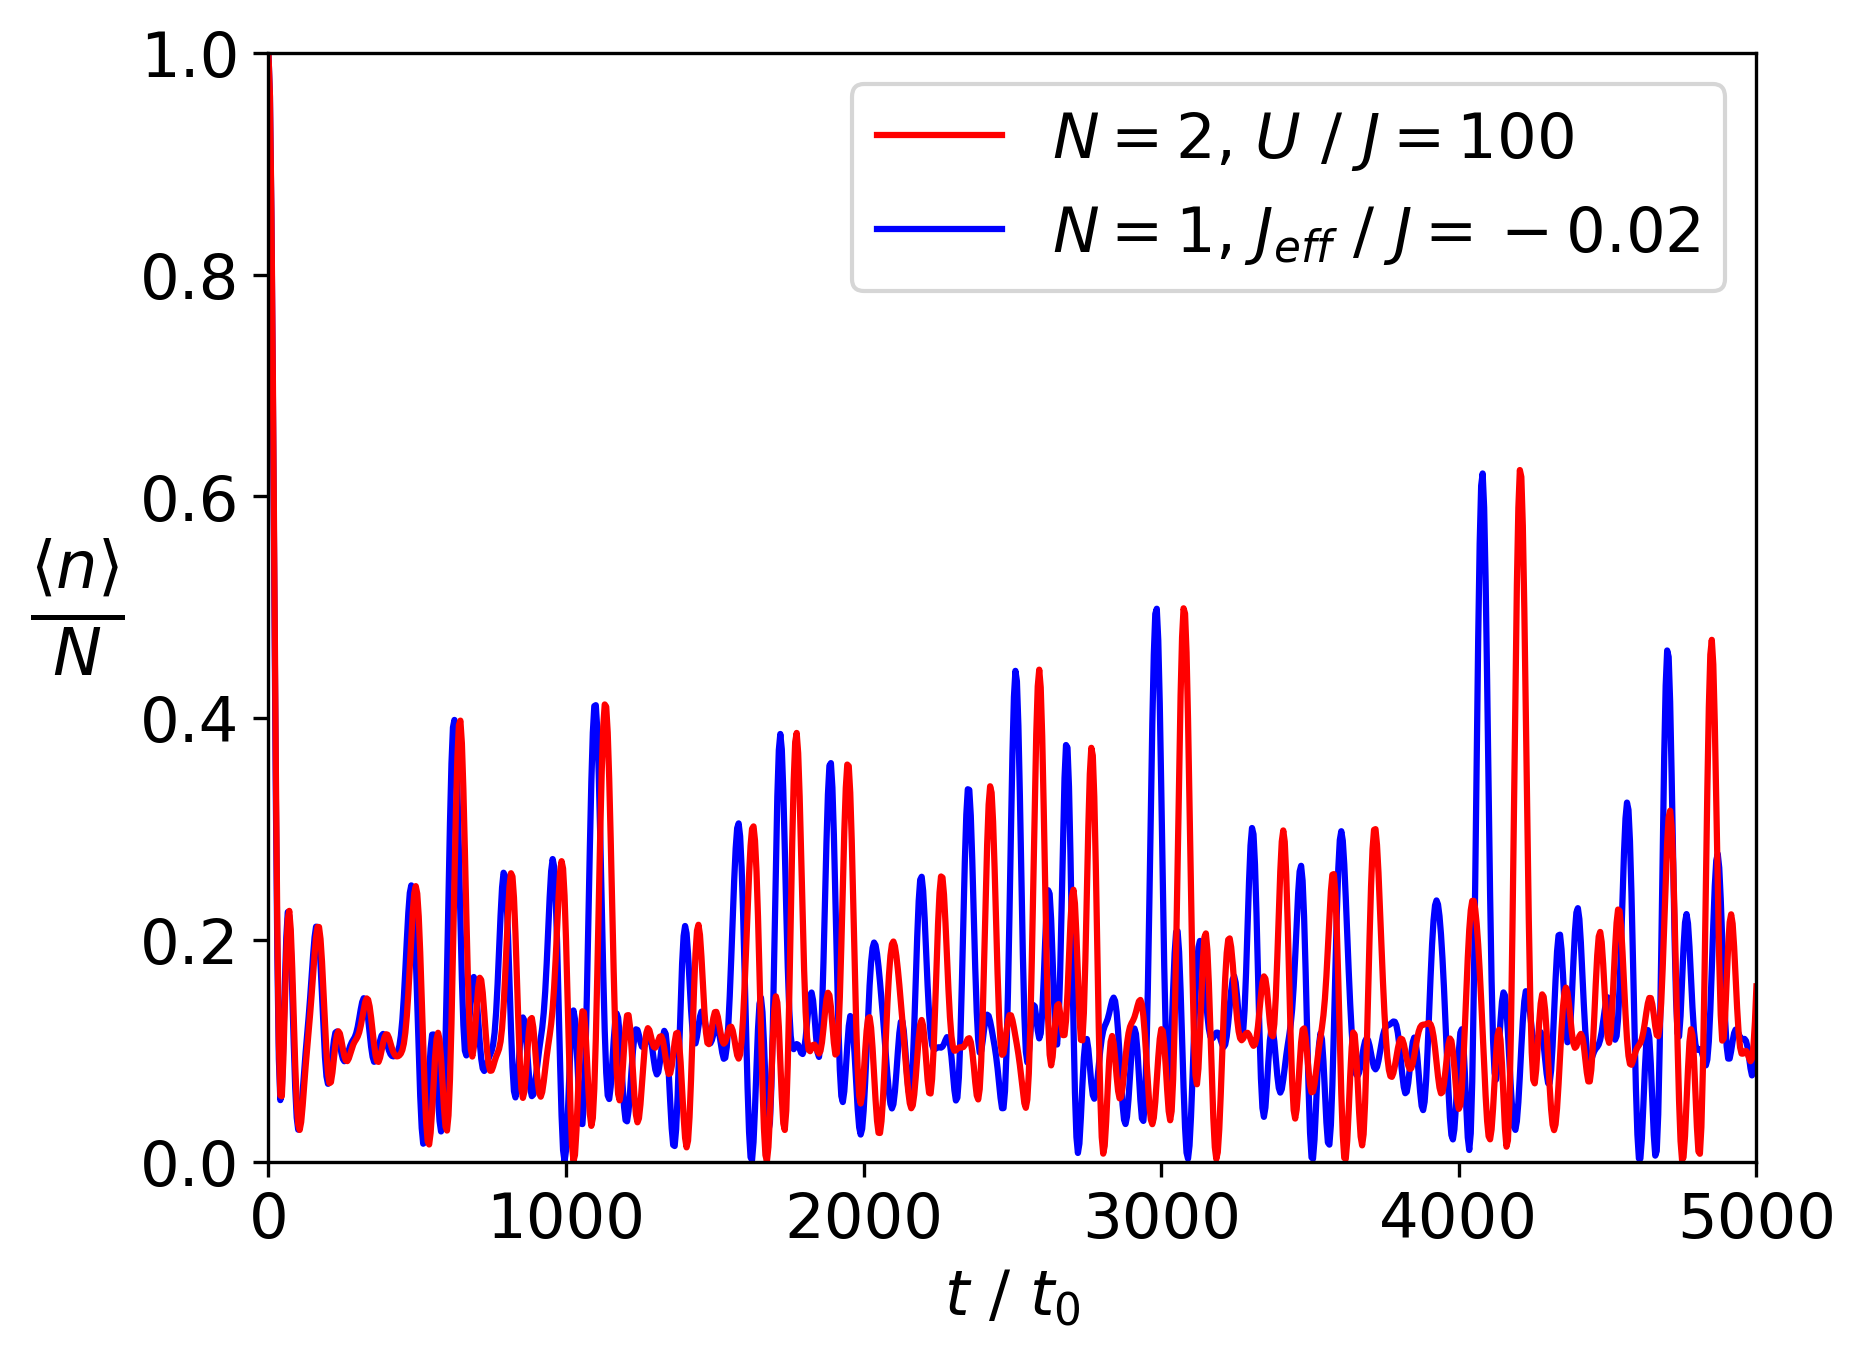
\includegraphics[height=5.6cm]{Figures/Doublon_SingleSite_Evolution}\label{Fig:Doublon_SingleSite_Evolution}}\hfill
    \sidesubfloat[]{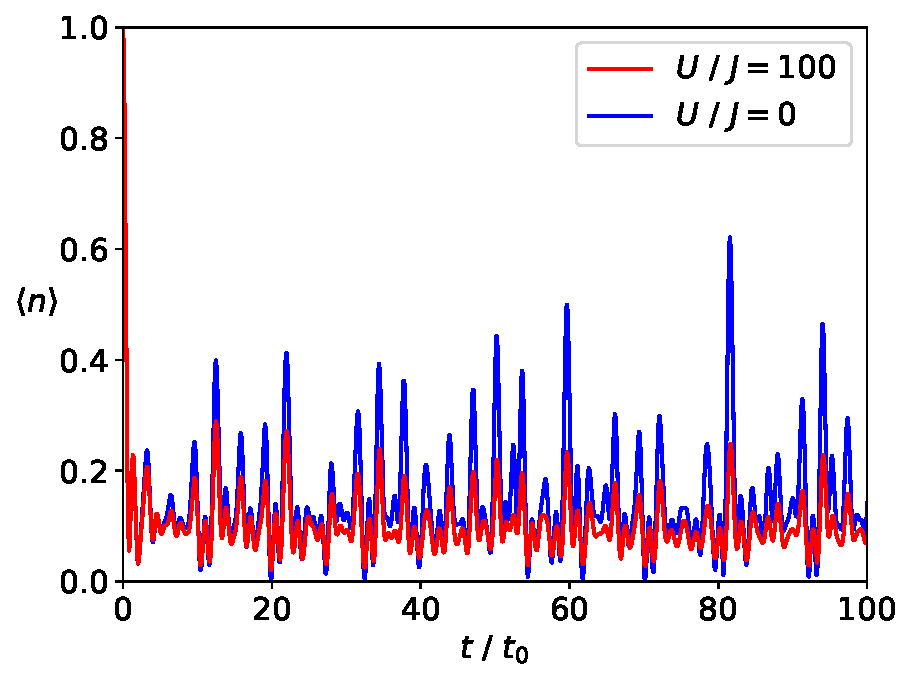
\includegraphics[height=5.6cm]{Figures/Scattering_Evolution}\label{Fig:Scattering_Evolution}}
    \setlength{\belowcaptionskip}{1cm}
    \caption{Dynamical behaviour of strongly-interacting systems. (a) Time-evolution of density in original site for a single-site initial state, for the strongly-interacting two-particle case, and as calculated using the effective single-particle model Eq. \ref{Eq:DoublonHamiltonian}. The density is normalized by the number of particles, $N$, to enable comparison of one- and two-particle data. (b) Time-evolution of density in one of the original sites, for particles initially on two different sites, for strongly- and non-interacting cases.}
    \label{Fig:Strong_Interaction_Real_Time}
\end{figure}

\text{ }

\subsection{Expected Separation}\label{Sec:Exp_Separation}

The expected particle separation is:
\begin{equation}
    \langle r \rangle = \sum_{(ij)}|c_{ij}(t)|^2|\textbf{r}_i-\textbf{r}_j|
\end{equation}
where $(ij)$ indicates the exclusion of permutations $ij \rightarrow ji$ to avoid double-counting, $c_{ij}(t)=\langle 0|b_{i}b_{j}|\Psi(t)\rangle$ (with an extra factor of $\frac{1}{\sqrt{2}}$ when $i=j$), and $|\textbf{r}_i-\textbf{r}_j|$ is the minimum distance between sites $i$ and $j$, taking account of the periodic boundary conditions. Fig. \ref{Fig:Separation_vs_t} shows $\langle r \rangle$ against time from simulations with the hexagon initial state. For all $U$, after an initial transient period, $\langle r \rangle$ fluctuates around a steady-state value. The time-averaged steady-state separation $\overline{\langle r \rangle}$ is plotted against $U$ in Fig. \ref{Fig:Separation_vs_U}. For weak interactions, $\overline{\langle r \rangle}<a$ and is independent of $U$; as predicted, the particles are bound closely together, for arbitrarily weak interaction strengths. For $U\gtrsim J$, the two-particle eigenstates are mixtures of the single-particle flat and dispersive bands, as discussed previously. The particles are therefore independently mobile, so $\overline{\langle r \rangle}$ increases. The large-$U$ value of $\overline{\langle r \rangle}$ is determined only by the lattice geometry, not correlations between the particles; it is on the order of the lattice width ($10\,a$) divided by 4, due to the periodic boundary conditions.

\vspace{1cm}

\begin{figure}[ht]
    \centering
    \sidesubfloat[]{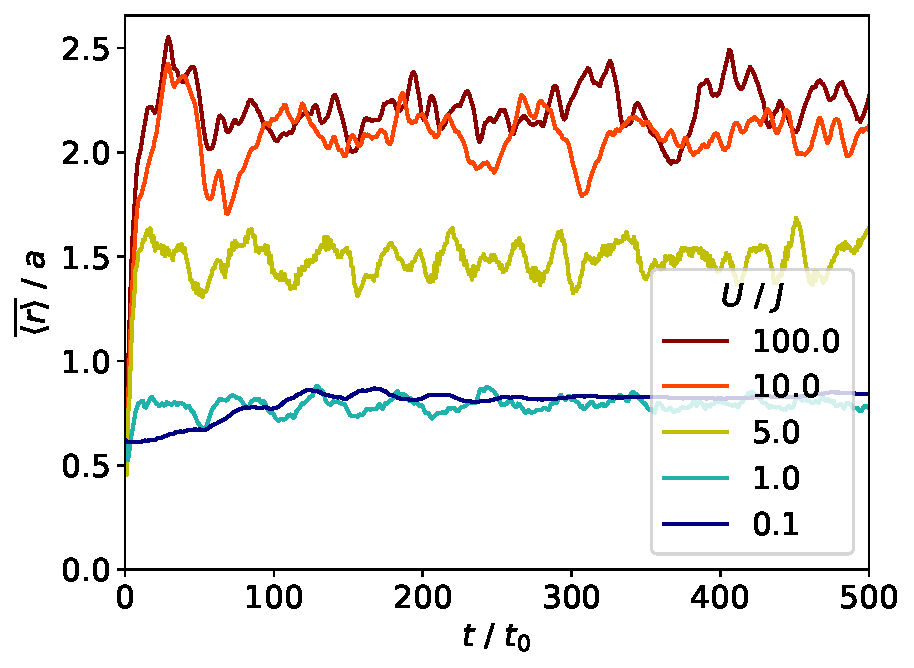
\includegraphics[height=5.6cm]{Figures/Separation_vs_t}\label{Fig:Separation_vs_t}}\hfill
    \sidesubfloat[]{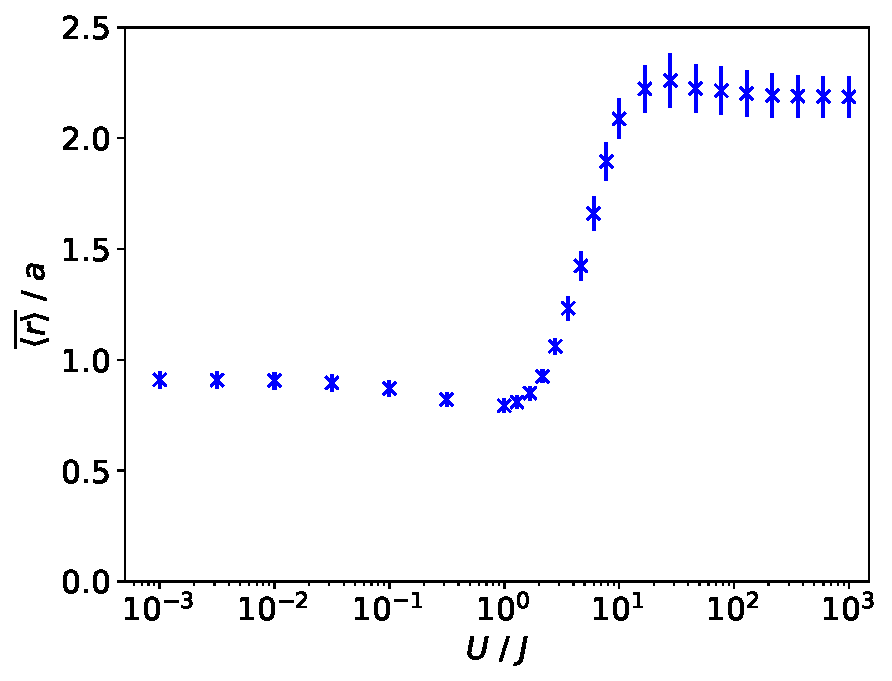
\includegraphics[height=5.6cm]{Figures/Separation_vs_U}\label{Fig:Separation_vs_U}}
    \caption{(a) Expected particle separation against time from simulations with the hexagon initial state, for various interaction strengths. (b) Time-averaged expected separation (after steady-state has been reached) against interaction strength. Error bars show standard deviations of the fluctuations.}
    \label{Fig:ParticleSeparation}
\end{figure}

\subsection{Radial Distribution Function}

Additional insight is available from the probability $P(r)$ that the particles occupy any state with sites separated by $r$:
\begin{equation}
    P(r) = \sum_{(ij)}|c_{ij}|^2 \delta_{r,|\textbf{r}_i-\textbf{r}_j|}
\end{equation}
where $\delta_{r,|\textbf{r}_i-\textbf{r}_j|}$ is the Kronecker delta; only discrete values of $r$ determined by the lattice are possible. The expected separation $\langle r \rangle$ is equal to $\sum_r rP(r)$. In fact, a more convenient quantity to interpret is the `radial distribution function' $g(r)$, defined as $P(r)$ divided by the number of basis states consisting of sites separated by $r$, $N(r)$:
\begin{equation}
    g(r) = \frac{P(r)}{N(r)}=\frac{\sum_{(ij)}|c_{ij}|^2 \delta_{r,|\textbf{r}_i-\textbf{r}_j|}}{\sum_{(ij)}\delta_{r,|\textbf{r}_i-\textbf{r}_j|}}
\end{equation}
With no correlations between particles, all basis states have an equal chance of being occupied; $g(r)$ is therefore constant, and equal to $1/N_{\text{states}}$.

For different initial states and interaction strengths, $g(r)$ was calculated at each evolution timestep. As with $\langle r \rangle$, $g(r)$ tends to a steady-state distribution after an initial transient period. Fig. \ref{Fig:RDFs} shows the time-averaged steady-state $g(r)$. With the particles initially on different sites (Fig. \ref{Fig:Separate_Sites_RDF}), a peak remains around $r=2\,a$. This is due to the stationary flat band density localised around each of the original sites, as in the single-particle simulations of Section \ref{Sec:SingleParticleResults}. Since the two sites are separated, the flat band eigenstates localised around each site do not overlap one another, and therefore have no interaction energy shift and remain stationary. For other values of $r$ and weak interactions, $g(r)$ is close to the constant value expected with no correlations between particles. For strong interactions, $g(r)$ is similar to the weak-interaction case for most values of $r$, except $g(r=0)\approx 0$; doublon states are inaccessible for this initial scattering state, as expected.

For the hexagon initial state (Fig. \ref{Fig:Hexagon_RDF}), for weak interactions $g(r)$ is largest around $r=0$, and decreases to almost 0 for $r\gtrsim a$. This supports Section \ref{Sec:Exp_Separation} in confirming that the particles are bound together as they move. For strong interactions, there is a peak at $r=0$ due to the initial occupancy of doublon states which are subsequently unable to separate. $g(r>0)$ is almost uniform, showing the absence of correlations between the particles away from $r=0$ in the scattering band. 

\begin{figure}[ht]
    \centering
    \sidesubfloat[]{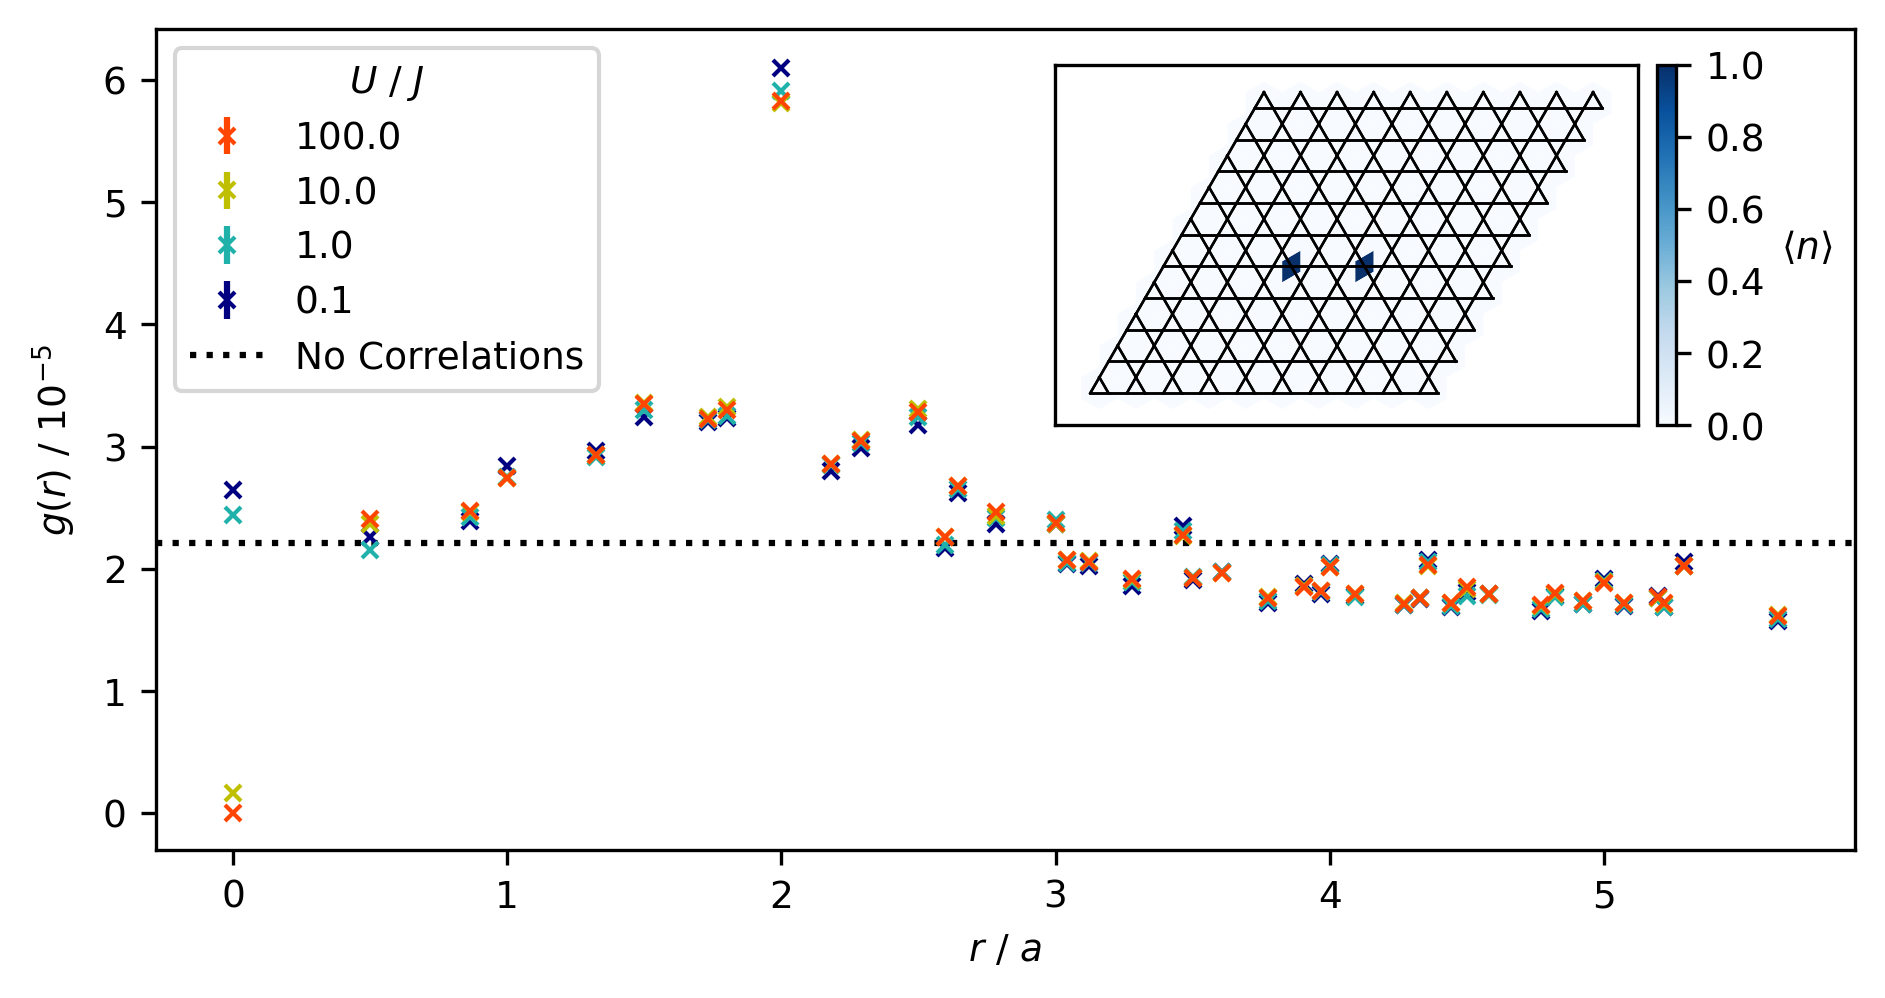
\includegraphics[width=0.96\textwidth]{Figures/Separate_Sites_RDF_with_inset_2}\label{Fig:Separate_Sites_RDF}}

    \sidesubfloat[]{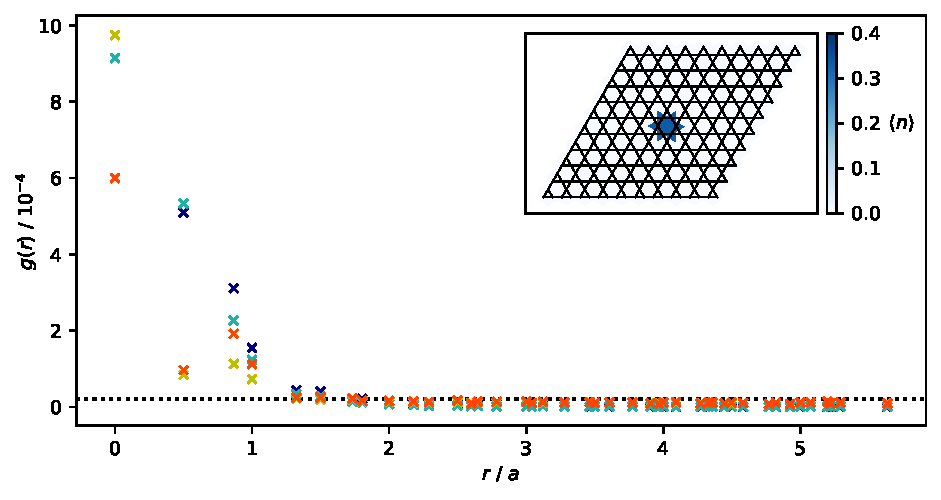
\includegraphics[width=0.96\textwidth]{Figures/Hexagon_RDF_with_inset_2}\label{Fig:Hexagon_RDF}}
    
    \caption{Time-averaged steady-state radial distribution functions for (a) particles initially on separate sites, and (b) the hexagon initial state. Insets show the initial density distributions. The legend in (a) applies to both plots. Error bars indicating the standard deviation of fluctuations in $g(r)$ are too small to be seen for most points.}
    \label{Fig:RDFs}
\end{figure}